\documentclass[11pt]{article}
% Reconstructed from the published note; revised October 7, 2026.
\usepackage[T1]{fontenc}
\usepackage{lmodern,microtype}
\usepackage[margin=1in]{geometry}
\usepackage{amsmath,amssymb,amsthm}
\usepackage{enumitem,tikz}
\usetikzlibrary{decorations.pathreplacing,arrows.meta}
\usepackage[colorlinks=true,linkcolor=blue!45!black,urlcolor=blue!45!black]{hyperref}
\hypersetup{pdftitle={Lebesgue's Criterion for Riemann Integrability},pdfauthor={Henry Shin},pdfsubject={A compactness proof of sufficiency and a direct proof of stability under continuous composition}}
\setlength{\parindent}{0pt}
\setlength{\parskip}{0.45em}
\setlist[itemize]{leftmargin=1.6em,itemsep=0.35em}
\newtheorem{theorem}{Theorem}
\newtheorem{corollary}[theorem]{Corollary}
\newcommand{\R}{\mathbb R}
\DeclareMathOperator{\osc}{osc}
\title{\vspace{-1.1cm}Lebesgue's Criterion for Riemann Integrability\\[0.2em]\large A Compactness Proof of Sufficiency}
\author{Henry Shin}
\date{April 30, 2026\\[0.25em]\small Revised October 7, 2026}
\begin{document}
\maketitle
\vspace{-0.6cm}
\begin{abstract}
A bounded function whose discontinuities form a set of measure zero is Riemann integrable. We prove this by covering the discontinuities with intervals of small total length and using continuity on the complement to control oscillation. A finite subcover yields a partition for which every term in the Darboux gap is controlled by one of these two estimates. The construction keeps track of cell endpoints, where bounds on open intervals alone would not suffice. A final application uses the same division of the Darboux sum to prove stability under continuous composition.
\end{abstract}

\section{The theorem and its proof}
Throughout, $a\leq b$. When $a=b$, the integral is zero; the proof below treats $a<b$.
\begin{theorem}[Lebesgue's criterion, sufficiency]
Let $f:[a,b]\to\R$ be bounded. If its set of discontinuities $E$ has Lebesgue measure zero, then $f$ is Riemann integrable on $[a,b]$.
\end{theorem}
\begin{proof}
\textbf{Step 1: Choose the two tolerances.}
Put $M=\sup_{x\in[a,b]}|f(x)|$. If $M=0$, the result is immediate. Assume $M>0$ and fix $\varepsilon>0$. We will construct a partition $P$ such that $U(f,P)-L(f,P)<\varepsilon$.

\textbf{Step 2: Cover the discontinuities.}
Since $E$ has measure zero, there are open intervals $(c_j,d_j)$ such that
\[
 E\subseteq\bigcup_{j=1}^{\infty}(c_j,d_j),
 \qquad \sum_{j=1}^{\infty}(d_j-c_j)<\frac{\varepsilon}{4M}.
\]
Write $U=\bigcup_j(c_j,d_j)$ and $K=[a,b]\setminus U$. The set $K$ is compact, and $f$ is continuous at each of its points, as a function on $[a,b]$.

\textbf{Step 3: Control oscillation on closed neighborhoods.}
For each $x\in K$, continuity gives $\delta_x>0$ such that
\[
 y\in[a,b],\quad |y-x|<2\delta_x
 \quad\Longrightarrow\quad
 |f(y)-f(x)|<\frac{\varepsilon}{4(b-a)}.
\]
Set $I_x=(x-\delta_x,x+\delta_x)$. If $y,z\in\overline{I_x}\cap[a,b]$, their distances from $x$ are at most $\delta_x<2\delta_x$. Thus
\[
 |f(y)-f(z)|\leq |f(y)-f(x)|+|f(x)-f(z)|
 <\frac{\varepsilon}{2(b-a)}.
\]
Taking a supremum over pairs gives the non-strict bound
\[
 \osc_{\overline{I_x}\cap[a,b]}f\leq\frac{\varepsilon}{2(b-a)}.
\]
Here $\osc_A f=\sup_A f-\inf_A f$ for a nonempty set $A$. The factor of two in the choice of radius ensures that the estimate includes the endpoints of $I_x$.

\begin{center}
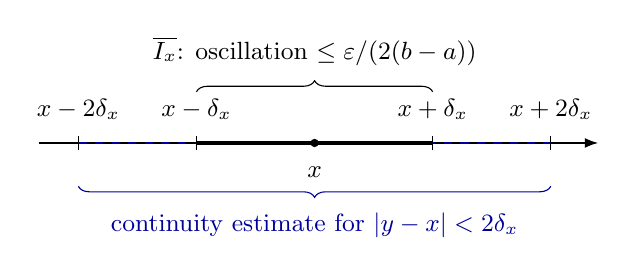
\begin{tikzpicture}[x=1cm,y=1cm,>=Latex,font=\small]
\draw[->] (-3.5,0)--(3.6,0);
\draw[blue!60!black,dashed,thick] (-3,0)--(3,0);
\draw[very thick] (-1.5,0)--(1.5,0);
\foreach \x/\lab in {-3/{x-2\delta_x},-1.5/{x-\delta_x},1.5/{x+\delta_x},3/{x+2\delta_x}}{
\draw (\x,-0.09)--(\x,0.09);\node[above=5pt] at (\x,0) {$\lab$};}
\fill (0,0) circle (1.5pt);\node[below=5pt] at (0,0) {$x$};
\draw[decorate,decoration={brace,amplitude=4pt}] (-1.5,0.65)--(1.5,0.65)
 node[midway,above=6pt] {$\overline{I_x}$: oscillation $\leq\varepsilon/(2(b-a))$};
\draw[decorate,decoration={brace,mirror,amplitude=4pt},blue!60!black] (-3,-0.55)--(3,-0.55)
 node[midway,below=6pt] {continuity estimate for $|y-x|<2\delta_x$};
\end{tikzpicture}
\end{center}
\textit{Figure 1.} The closed interval $\overline{I_x}$ lies inside the neighborhood where continuity controls the values of $f$. All estimates are restricted to $[a,b]$.

\textbf{Step 4: Pass to a finite cover.}
The family $\{I_x:x\in K\}\cup\{(c_j,d_j):j\geq1\}$ covers $[a,b]$. By compactness it has a finite subcover
\[
 \mathcal F=\{I_{x_1},\ldots,I_{x_n}\}\cup
 \{(c_{j_1},d_{j_1}),\ldots,(c_{j_m},d_{j_m})\}.
\]
Either part may be empty. Let $S$ consist of $a,b$ and every endpoint of an interval in $\mathcal F$ that lies in $(a,b)$. In increasing order these points form a partition
\[
 P=\{t_0,\ldots,t_N\},\qquad a=t_0<t_1<\cdots<t_N=b.
\]

\textbf{Step 5: Locate each open cell in the cover.}
Each cell $(t_{k-1},t_k)$ is contained in at least one interval of $\mathcal F$. To see this, choose $y\in(t_{k-1},t_k)$ and an interval $(A,B)\in\mathcal F$ containing $y$. No endpoint of $\mathcal F$ lies inside the cell, so $A\leq t_{k-1}$ and $B\geq t_k$. Hence $(t_{k-1},t_k)\subseteq(A,B)$.

\begin{center}
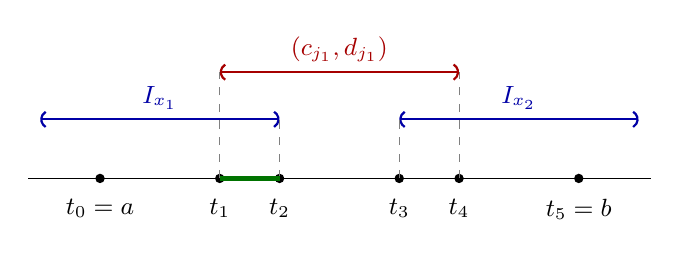
\begin{tikzpicture}[x=0.76cm,y=0.75cm,font=\small]
\draw (-0.2,0)--(10.2,0);
\draw[blue!65!black,thick,{Parenthesis}-{Parenthesis}] (0,1)--(4,1) node[midway,above] {$I_{x_1}$};
\draw[red!65!black,thick,{Parenthesis}-{Parenthesis}] (3,1.8)--(7,1.8) node[midway,above] {$(c_{j_1},d_{j_1})$};
\draw[blue!65!black,thick,{Parenthesis}-{Parenthesis}] (6,1)--(10,1) node[midway,above] {$I_{x_2}$};
\foreach \x/\lab in {1/{t_0=a},3/{t_1},4/{t_2},6/{t_3},7/{t_4},9/{t_5=b}}{
\fill (\x,0) circle (1.7pt);\node[below=4pt] at (\x,0) {$\lab$};}
\foreach \x/\y in {3/1.8,4/1,6/1,7/1.8}{\draw[dashed,gray] (\x,0)--(\x,\y);}
\draw[green!45!black,line width=2pt] (3,0)--(4,0);
\end{tikzpicture}
\end{center}
\textit{Figure 2.} The cover endpoints determine the partition. Covering intervals may overlap: the highlighted cell lies in two of them. The open partition cells themselves are disjoint.

\textbf{Step 6: Estimate the Darboux gap.}
Put $\Delta t_k=t_k-t_{k-1}$ and $\omega_k=\osc_{[t_{k-1},t_k]}f$. Divide the indices into two disjoint classes:
\begin{itemize}
\item $G$: those $k$ for which $(t_{k-1},t_k)\subseteq I_{x_i}$ for some $i$;
\item $B$: all remaining indices, whose open cells must therefore lie in one of the selected intervals $(c_{j_s},d_{j_s})$.
\end{itemize}
For $k\in G$, taking closures gives $[t_{k-1},t_k]\subseteq\overline{I_{x_i}}\cap[a,b]$. By Step 3,
\[
 \sum_{k\in G}\omega_k\Delta t_k
 \leq\frac{\varepsilon}{2(b-a)}\sum_{k\in G}\Delta t_k
 \leq\frac{\varepsilon}{2}.
\]
For $k\in B$, boundedness gives $\omega_k\leq2M$. The corresponding open cells are pairwise disjoint and lie in $U$, so additivity of length on disjoint intervals and countable subadditivity give
\[
 \sum_{k\in B}\Delta t_k
 \leq\sum_{j=1}^{\infty}(d_j-c_j)<\frac{\varepsilon}{4M}.
\]
Their endpoints need not lie in $U$: the bound $2M$ holds on every closed cell. Consequently,
\[
 \sum_{k\in B}\omega_k\Delta t_k<\frac{\varepsilon}{2}.
\]
Adding the two estimates yields
\[
 U(f,P)-L(f,P)=\sum_{k=1}^{N}\omega_k\Delta t_k<\varepsilon.
\]
The Darboux criterion proves the theorem.
\end{proof}

\section{Two ways to control the same sum}
Each term of the Darboux gap is a product of an oscillation and an interval length. The proof uses this in two complementary ways. On the cells indexed by $G$, continuity controls the oscillation while their total length is at most $b-a$. On those indexed by $B$, boundedness controls the oscillation while the measure-zero hypothesis makes their total length small. Assigning each cell to exactly one class makes the estimates compatible even when the covering intervals overlap.

The argument depends on the total length of a cover, not on how densely the discontinuities are distributed. For example, Thomae's function on $[0,1]$ is defined by $T(p/q)=1/q$ for a rational in lowest terms with $q>0$, and $T(x)=0$ for irrational $x$. For any fixed bound on $q$, only finitely many such rationals lie in $[0,1]$. This proves continuity at every irrational point; density of the irrationals proves discontinuity at every rational point. Its discontinuity set is therefore dense and countable, but has measure zero, so the theorem applies.

Uncountable discontinuity sets are also possible. The indicator of the middle-thirds Cantor set on $[0,1]$ is discontinuous exactly on that set: it is locally constant on the complement, while every neighborhood of a point in the set meets the complement. Since the Cantor set has measure zero, its indicator is Riemann integrable as well.

\clearpage
\section{Continuous composition}
The same division of the Darboux sum proves the following closure property directly. This argument uses neither direction of Lebesgue's criterion.
\begin{corollary}
If $f:[a,b]\to[c,d]$ is Riemann integrable and $g:[c,d]\to\R$ is continuous, then $g\circ f$ is Riemann integrable on $[a,b]$.
\end{corollary}
\begin{proof}
The case $a=b$ is immediate. Assume $a<b$ and put $\ell=b-a>0$. Continuity on the compact interval $[c,d]$ gives a constant $B>0$ with $|g(t)|\leq B$. Given $\varepsilon>0$, uniform continuity gives $\delta>0$ such that
\[
 u,v\in[c,d],\quad |u-v|<\delta
 \quad\Longrightarrow\quad |g(u)-g(v)|<\frac{\varepsilon}{2\ell}.
\]
For a partition $P$, put $I_i=[x_{i-1},x_i]$, $\Delta x_i=x_i-x_{i-1}$, and $\omega_i(h)=\osc_{I_i}h$. By the Darboux criterion for $f$, choose $P$ with
\[
 D_f(P):=U(f,P)-L(f,P)=\sum_i\omega_i(f)\Delta x_i
 <\frac{\varepsilon\delta}{4B}.
\]
On cells with $\omega_i(f)<\delta$, every pair of values of $f$ differs by less than $\delta$. Hence $\omega_i(g\circ f)\leq\varepsilon/(2\ell)$, and these cells contribute at most $\varepsilon/2$ to the Darboux gap for $g\circ f$.

The remaining cells have $\omega_i(f)\geq\delta$, so their total length is at most $D_f(P)/\delta<\varepsilon/(4B)$. Since $\omega_i(g\circ f)\leq2B$ on every cell, they contribute strictly less than $\varepsilon/2$. Therefore
\[
 U(g\circ f,P)-L(g\circ f,P)<\varepsilon.
\]
The composition is bounded by $B$, so the Darboux criterion finishes the proof.
\end{proof}
\end{document}
